\chapter{Метод анализа генетических данных для оценки региональных различий адаптации к климатическим условиям}\label{ch:ch3}

\section{Входные данные}\label{sec:ch3/sec1}

Для анализа генетических данных используется информация об однонуклеотидных полиморфизмах (SNP), распределённых по всему геному человеческого организма. Наиболее обширной базой данных генетических вариантов является проект <<1000 геномов>> \autocite{1000genomes2015, Sudmant2015}, целью которого было найти большинство генетических вариантов с частотой не менее $1~\%$ в изучаемых популяциях и создать Международный ресурс геномных образцов (International Genome Sample Resource --- IGSR). В рамках данного проекта были использованы достижения в области технологии секвенирования, что резко снизило его стоимость. Это был первый проект по секвенированию геномов большого числа людей, чтобы собрать большую базу данных генетических вариаций человека. Секвенирование оставалось слишком дорогим для проведения глубокого анализа многих образцов, изучаемых в рамках проекта. Однако, любая конкретная область генома обычно содержит ограниченное количество гаплотипов. Данные были объединены по образцам, чтобы обеспечить эффективное обнаружение большинства вариантов в изучаемом географическом регионе. В рамках проекта каждый образец секвенировался до 4-кратного покрытия генома; на этой глубине секвенирование не может обнаружить все варианты в каждом образце, но может позволить выявить большинство вариантов с частотами всего $1~\%$. На заключительном этапе проекта были объединены данные из 2504 образцов, чтобы обеспечить высокоточное определение генотипов в каждом образце на всех вариативных участках. Образцы для проекта <<1000 геномов>> анонимны и не имеют связанных медицинских или фенотипических данных. Проект придерживается самооценки этнической принадлежности и пола. Во время сбора образцов все участники заявили, что они здоровы. Текущие образцы проекта <<1000 геномов>> не отражают все популяции (список доступных популяций указан в Таблице~\ref{tab:populations}), однако, его целью является обеспечение максимально возможного разнообразия населения. 

\begin{table} [htbp]
	\centering
	\begin{threeparttable}
		\caption{Популяции, представленные в проекте <<1000 геномов>>}%
		\label{tab:populations}%
		\begin{SingleSpace}
			\begin{tabular}{| c | c | c |}
				\hline
				Код 	& Описание 							& Суперпопуляция \\ \hline
				CHB 	& Хань в Пекине, Китай 				& Восточная Азия \\ \hline
				JPT 	& Японцы в Токио, Япония 			& Восточная Азия \\ \hline
				CHS 	& Хань на юге Китая 				& Восточная Азия \\ \hline
				CDX 	& Дай в Сишуанбаньна, Китай 		& Восточная Азия \\ \hline
				KHV 	& Кин в Хошимине, Вьетнам			& Восточная Азия \\ \hline
				CEU 	& \thead{Жители Юты северного и западноевропейского \\ происхождения} 		& Европа \\ \hline
				TSI 	& Тосканцы в Италии	 				& Европа \\ \hline
				FIN 	& Финны в Финляндии 				& Европа \\ \hline
				GBR 	& Британцы в Англии и Шотландии		& Европа \\ \hline
				IBS 	& Иберийское население в Испании	& Европа \\ \hline
				YRI 	& Йоруба в Ибадане, Нигерия			& Африка \\ \hline
				LWK 	& Лухья в Вебуе, Кения		 		& Африка \\ \hline
				GWD 	& Гамбийцы в западных районах Гамбии										& Африка \\ \hline
				MSL 	& Менде в Сьерра-Леоне				& Африка \\ \hline
				ESN 	& Ишан в Нигерии	 				& Африка \\ \hline
				ASW 	& \thead{Американцы африканского происхождения \\ на юго-западе США}		& Африка \\ \hline
				ACB 	& Вест-индские негры на Барбадосе 	& Африка \\ \hline
				MXL 	& \thead{Мексиканское население Лос-Анджелеса, \\ США} 						& Америка (смешанные) \\ \hline
				PUR 	& Пуэрториканцы в Пуэрто-Рико		& Америка (смешанные) \\ \hline
				CLM 	& Колумбийцы в Медельине, Колумбия 	& Америка (смешанные) \\ \hline
				PEL 	& Перуанцы в Лиме, Перу				& Америка (смешанные) \\ \hline
				GIH 	& Гуджаратцы в Хьюстоне, штат Техас & Южная Азия \\ \hline
				PJL 	& Панджабцы в Лахоре, Пакистан		& Южная Азия \\ \hline
				BEB 	& Бенгальцы в Бангладеше 			& Южная Азия \\ \hline
				STU 	& Ланкийские тамилы	в Великобритании										& Южная Азия \\ \hline
				ITU 	& Индийские телугу в Великобритании	& Южная Азия \\ \hline
			\end{tabular}%
		\end{SingleSpace}
	\end{threeparttable}
\end{table}

Отбор проб для проекта <<1000 геномов>> осуществляется в соответствии со следующими критериями:
\begin{itemize}
	\item Все образцы крови взяты у взрослых субъектов.
	\item Для получения 100 неродственных клеточных линий популяции, первичный материал был собран как минимум от 130 неродственных субъектов.
	\item Получены линии <<бессмертных>> клеток, которые можно использовать для получения практически неограниченных количеств ДНК.
	\item Образцы генотипированы с использованием массива генотипов высокой плотности с более чем 500000 маркеров.
\end{itemize}

Информация об однонуклеотидных полиморфизмах сохраняется в формате VCF (Variant Call Format) --- это формат текстового файла, используемого в биоинформатике для хранения генетических вариаций последовательностей генов. Формат был разработан с появлением крупных проектов секвенирования и фенотипирования ДНК, таких как проект <<1000 геномов>>. Файл формата VCF обязательно включает заголовок, который содержит метаданные, описывающие тело файла. Строки заголовков начинаются с символа $\#$, специальные ключевые слова в заголовке обозначаются $\#\#$. Тело файла представляется собой табулированную таблицу, содержащую 8 обязательных столбцов и неограниченное количество дополнительных столбцов. Когда используются дополнительные столбцы, первый дополнительный столбец используется для описания формата данных в следующих столбцах. Обязательные столбцы:
\begin{enumerate}
	\item CHROM --- имя хромосомы, в которой располагается полиморфизм. 
	\item POS --- номер позиции, в которой находится полиморфизм, отсчитываемый от 1.
	\item ID --- идентификатор полиморфизма, например, идентификатор rs или, если он неизвестен, ".".
	\item REF --- референсная аллель в данной позиции.
	\item ALT --- список альтернативных аллелей в данной позиции.
	\item QUAL --- оценка качества, связанная с данными аллелями.
	\item FILTER --- флаг, указывающий, какой из заданного набора фильтров был применён.
	\item INFO --- список пар (полей) ключ-значение, описывающих полиморфизм. 
	\item FORMAT --- (необязательный) расширяемый список полей для описания образцов.
	\item SAMPLES --- значения полей, перечисленных в FORMAT, для каждого (необязательного) образца, описанного в файле.
\end{enumerate}

Известно, что климат играет важную роль в формировании геномного разнообразия популяций, влияя на несколько человеческих черт, таких как размер тела, пигментация кожи, расход энергии, метаболизм питательных веществ \autocite{Sturm2012, Hancock2011adaptations, Quagliarello2017}. В то же время митохондрии имеют решающее значение для выделения тепла во многих организмах и для их метаболической роли в генерации АТФ. В соответствии с этим для проверки результатов работы предлагаемых алгоритмов использовалась часть данных генетических вариаций проекта <<1000 геномов>>, соответствующих репрезентативным популяциям европейского происхождения из разных широт (Рисунок~\ref{fig:europe_map}) --- GBR (Британцы в Англии и Шотландии), FIN (Финны в Финляндии), TSI (Тосканцы в Италии).

\begin{figure}[ht]
	\centerfloat{
		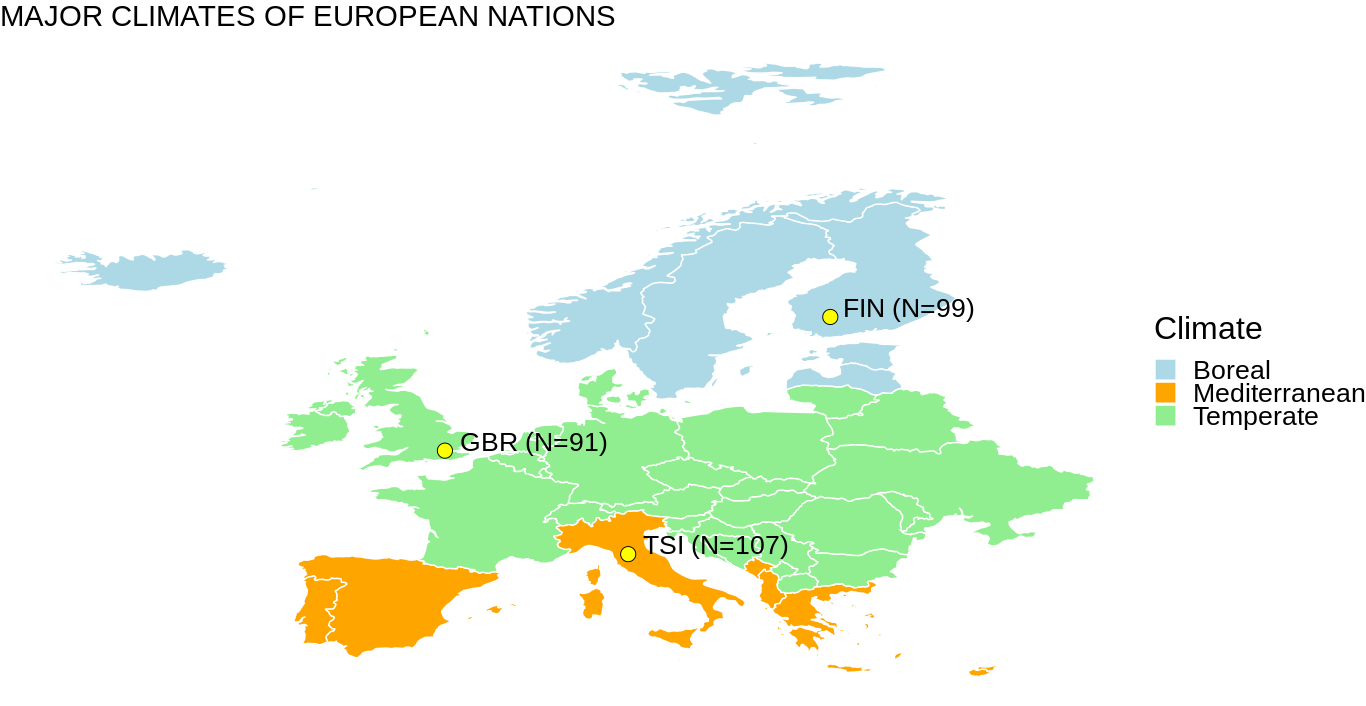
\includegraphics[scale=0.3]{europe_map.png}
	}
	\caption[Карта Европы с рассматриваемыми популяциями и различными климатическими регионами.]{Карта Европы с рассматриваемыми популяциями и различными климатическими регионами: субарктический (синий), средиземноморский (оранжевый) и умеренный (зелёный).}\label{fig:europe_map}
\end{figure}

\section{Подход к уменьшению размерности входных данных}\label{sec:ch3/sec2}

Основным объектом исследования являются однонуклеотидные полиморфизмы генома человека, количество которых составляет примерно 5.000.000 в ядерном геноме человека и 3000 --- в митохондриальном. При рассмотрении парных митохондриально-ядерных взаимодействий количество исследуемых пар составляет $1 \cdot 10^{10}$, что затрудняет применение классических статистических методов. Одним из способов снижения размерности является рассмотрение некоторого подмножества ядерных генов с определённой функциональностью, например, связанных с адаптацией к определённым климатическим условиям. В дальнейшем будем рассматривать подмножество из 28 ядерных генов, которые ранее были связаны с адаптацией организма человека к холоду \autocite{Sazzini2014}. Поскольку количество митохондриальных генов невелико (13), и количество однонуклеотидных полиморфизмов в них не превышает 3000, будем рассматривать их полностью. В Таблицах~\ref{tab:snp_mt} и \ref{tab:snp_nuc} представлены рассматриваемые митохондриальные и ядерные гены соответственно, а также количество однонуклеотидных полиморфизмов (SNP) в них.

\begin{table} [htbp]
	\centering
	\begin{threeparttable}
		\caption{Количество однонуклеотидных полиморфизмов (SNP) в митохондриальных генах}%
		\label{tab:snp_mt}%
		\begin{SingleSpace}
			\begin{tabular}{| c | c | c |}
				\hline
				Ген & Хромосома & Количество SNP \\ \hline
				MT-ND3        & MT                  & 77             \\ \hline
				MT-ATP6       & MT                  & 226            \\ \hline
				MT-ATP8       & MT                  & 73             \\ \hline
				MT-CO1        & MT                  & 319            \\ \hline
				MT-CO2        & MT                  & 152            \\ \hline
				MT-CO3        & MT                  & 182            \\ \hline
				MT-CYB        & MT                  & 326            \\ \hline
				MT-ND1        & MT                  & 218            \\ \hline
				MT-ND2        & MT                  & 236            \\ \hline
				MT-ND4        & MT                  & 291            \\ \hline
				MT-ND5        & MT                  & 408            \\ \hline
				MT-ND6        & MT                  & 128            \\ \hline
				MT-RNR1       & MT                  & 118            \\ \hline
				\multicolumn{2}{|l|}{Всего} 		& 2754		     \\ \hline
			\end{tabular}%
		\end{SingleSpace}
	\end{threeparttable}
\end{table}

\begin{table} [htbp]
	\centering
	\begin{threeparttable}
		\caption{Количество однонуклеотидных полиморфизмов (SNP) в рассматриваемых ядерных генах}%
		\label{tab:snp_nuc}%
		\begin{SingleSpace}
			\begin{tabular}{| c | c | c |}
				\hline
				Ген & Хромосома & Количество SNP \\ \hline
				ADRA1A        & 11                  & 7311           \\ \hline
				ADRB3         & 8                   & 203            \\ \hline
				CIDEA         & 18                  & 1445           \\ \hline
				CREB1         & 2                   & 4353           \\ \hline
				DIO2          & 14                  & 10223          \\ \hline
				FTO           & 16                  & 23729          \\ \hline
				HOXC4         & 12                  & 1801           \\ \hline
				HOXA1         & 7                   & 149            \\ \hline
				LIPE          & 19                  & 1485           \\ \hline
				LEP           & 7                   & 863            \\ \hline
				LEPR          & 1                   & 11705          \\ \hline
				NRF1          & 7                   & 6949           \\ \hline
				NRIP1         & 21                  & 753            \\ \hline
				PLIN1         & 15                  & 865            \\ \hline
				PLIN2         & 9                   & 2751           \\ \hline
				PLIN3         & 19                  & 2141           \\ \hline
				PLIN5         & 19                  & 999            \\ \hline
				PPARG         & 3                   & 7539           \\ \hline
				PPARGC1A      & 4                   & 5581           \\ \hline
				PPARGC1B      & 5                   & 7307           \\ \hline
				PRDM16        & 1                   & 28237          \\ \hline
				PRKAR1A       & 17                  & 1869           \\ \hline
				PRKAR2A       & 3                   & 4663           \\ \hline
				PRKAR1B       & 7                   & 14603          \\ \hline
				PRKAR2B       & 7                   & 6691           \\ \hline
				UCP1          & 4                   & 369            \\ \hline
				UCP2          & 11                  & 517            \\ \hline
				UCP3          & 11                  & 587            \\ \hline
				\multicolumn{2}{|l|}{Всего} 		& 155688	     \\ \hline
			\end{tabular}%
		\end{SingleSpace}
	\end{threeparttable}
\end{table}

Рассмотрение всех оставшихся митохондриально-ядерных комбинаций SNP по-прежнему представляет собой задачу огромной размерности. То есть, в лучшем случае митохондриальный ген ATP8 и ядерный ген HOXA1 дадут $73 \times 149 = 10877$ митохондриально-ядерных пар SNP, тогда как MT-ND5 и PRDM16 дадут $408 \times 28237 = 11520696$ митохондриально-ядерных пар SNP, общее количество пар SNP превышает $1 \cdot 10^{8}$. Для того, чтобы уменьшить общее количество рассматриваемых комбинаций SNP, была разработана вычислительная процедура усреднения информации об однонуклеотидных полиморфизмах в рамках каждого рассматриваемого гена.

Рассмотрим три основных типа экспериментов в зависимости от значений, принимаемыми однонуклеотидными полиморфизмами --- митохондриальная ДНК (2 варианта), ядерная ДНК (3 варианта), митохондриально-ядерные взаимодействия ДНК (6 вариантов). Сначала рассмотрим только митохондриальную ДНК, однонуклеотидные полиморфизмы в которой имеют один из двух вариантов --- 0 или 1. Количество вариаций для каждого из рассматриваемых субъектов равно 2754.

Алгоритм уменьшения размерности задачи для митохондриальных генов предполагает выполнение следующих шагов:
\begin{enumerate}
	\item Исключаются из рассмотрения такие однонуклеотидные полиморфизмы, которые не меняются среди всех рассматриваемых популяций (имеют значение либо 0, либо 1 для всех субъектов) --- они не несут популяционно-специфической информации.
	\item Одна из рассматриваемых популяций фиксируется как референсная. Относительно неё будут проводиться дальнейшие вычисления. Конкретный выбор популяции не имеет значения. В данной популяции для каждого из 13 митохондриальных генов вычисляется частота наблюдения каждого из вариантов SNP (0 или 1). Пусть далее $K$ --- количество SNP в гене $Gene N$, а $i = 1, 2, \cdots, K$. Тогда частоты вариантов 0 ($f_{Gene N}^{ref} (0)$) и 1 ($f_{Gene N}^{ref} (0)$) для гена $Gene N$ в референсной популяции будут равны:
	\begin{equation}
	\label{eq:f_ref_mt}
	\begin{gathered}
	f_{Gene N}^{ref} (0) = \frac{k_0}{K},\\
	f_{Gene N}^{ref} (1) = \frac{k_1}{K},
	\end{gathered}
	\end{equation}
	где $k_0$ --- количество вариантов 0 в гене $Gene N$, $k_1$ --- количество вариантов 1 в гене $Gene N$.
	\item Для каждого субъекта во всех рассматриваемых популяциях вычисляется частотная метрика каждого гена как среднее расстояние до референсной популяции. Для каждого гена в каждой популяции определяется расстояние по средней частоте мутаций как $\left(1 - f_{Gene N}^{ref} (0)\right)$. Если данное расстояние близко к 0, то среднее количество мутаций в данной популяции в данном гене близко к референсной популяции, если расстояние близко к 1 --- среднее количество мутаций в данном гене в данной популяции значительно отличается от референсной популяции. Вычисляется среднее значение частотной метрики в соответствии с формулой:
	\begin{equation}
	\label{eq:f_mt}
		\begin{gathered}
		f_{Gene N} (0) = \frac{\sum_{SNP_i\,in\,Gene N} \left(1 - f_{Gene N}^{ref} (0)\right)}{K},\\
		f_{Gene N} (1) = \frac{\sum_{SNP_i\,in\,Gene N} \left(1 - f_{Gene N}^{ref} (1)\right)}{K}.
		\end{gathered}
	\end{equation}
	\item Количество вариаций для каждого из рассматриваемых субъектов теперь равно количеству митохондриальных генов --- 13. Для дальнейшего анализа используются полученные значения метрик.
\end{enumerate}

Далее рассмотрим только ядерную ДНК, однонуклеотидные полиморфизмы в которой имеют один из трёх вариантов --- $0|0$, $0|1$ ($1|0$) или $1|1$. Количество вариаций для каждого из рассматриваемых субъектов равно 115688. Алгоритм уменьшения размерности задачи для рассматриваемых ядерных генов предполагает выполнение тех же шагов, за исключением того, что количество вычисляемых частот теперь будет равно 3, а итоговое количество вариаций для каждого из субъектов равно количеству рассматриваемых ядерных генов --- 28.

Рассмотрим наиболее общий случай взаимодействия митохондриальной и ядерной ДНК. При этом пары однонуклеотидных полиморфизмы имеют один из шести парных вариантов, где первый элемент идёт от митохондриальной ДНК, второй идёт от ядерной ДНК --- $0 + 0|0$, $0 + 0|1$ ($0 + 1|0$), $0 + 1|1$, $1 + 0|0$, $1 + 0|1$ ($1 + 1|0$), $1 + 1|1$. Количество пар вариаций для каждого из рассматриваемых субъектов превышает $1 \cdot 10^{8}$.

Алгоритм уменьшения размерности задачи для общего случая взаимодействия митохондриальных и ядерных генов предполагает выполнение следующих шагов:
\begin{enumerate}
	\item Исключаются из рассмотрения такие пары однонуклеотидных полиморфизмов, у которых оба элемента не меняются среди всех рассматриваемых популяций.
	\item Одна из рассматриваемых популяций фиксируется как референсная, относительно неё будут проводиться дальнейшие вычисления. В данной популяции для каждой из пар генов, где для определённости первый ген --- митохондриальный, второй --- ядерный, вычисляется частота наблюдения каждого из вариантов пар SNP. Пусть далее $M$ --- количество митохондриальных SNP в митохондриальном гене $mtGene M$, а $i = 1, 2, \cdots, M$; $N$ --- количество ядерных SNP в ядерном гене $nucGene N$, а $j = 1, 2, \cdots, N$. Тогда частота парного варианта $var$ для пары генов $mtGene M-nucGene N$ в референсной популяции будут равны:
	\begin{equation}
	\label{eq:f_ref_mt_nuc}
	f_{mtGene M-nucGene N}^{ref} (var) = \frac{k_{var}}{M\cdot N},
	\end{equation}
	где $k_{var}$ --- количество пар варианта $var$ в паре генов $mtGene M-nucGene N$.
	\item Для каждого субъекта во всех рассматриваемых популяциях вычисляется частотная метрика каждой пары генов как среднее расстояние до референсной популяции. Для каждой пары генов в каждой популяции определяется расстояние по средней частоте мутаций как $\left(1 - f_{mtGene M-nucGene N}^{ref} (var)\right)$. Если данное расстояние близко к 0, то среднее количество мутаций в данной популяции в данной паре генов близко к референсной популяции, если расстояние близко к 1 --- среднее количество мутаций в данной паре генов в данной популяции значительно отличается от референсной популяции. Вычисляется среднее значение частотной метрики в соответствии с формулой:
	\begin{equation}
	\label{eq:f_mt_nuc}
	\begin{gathered}
	f_{mtGene M-nucGene N} (var) =\\ \frac{\sum_{SNP_i\,in\,mtGene M, SNP_j\,in\,nucGene N} \left(1 - f_{mtGene M-nucGene N}^{ref} (var)\right)}{M\cdot N}.
	\end{gathered}
	\end{equation}
	\item Количество вариаций для каждого из рассматриваемых субъектов теперь равно количеству пар взаимодействий митохондриальных и ядерных генов --- 364. Для дальнейшего анализа используются полученные значения метрик.
\end{enumerate}

\section{Описание алгоритма анализа генетических данных}\label{sec:ch3/sec3}

Опишем алгоритм для определения митохондриально-ядерных взаимодействий, специфичных для популяций, проживающих в конкретных географических регионах и связанных с адаптацией к определённым климатическим условиям. Предполагается, что в качестве входа используются данные однонуклеотидных полиморфизмов, принадлежащих митохондриальной и ядерной ДНК, принадлежащие субъектам из различных популяций. Подробное описание входных данных представлено в Разделе~\ref{sec:ch3/sec1}.

Алгоритм предполагает выполнение следующих шагов: 
\begin{enumerate}
	\item Поскольку исходные данные представляют собой пары однонуклеотидных полиморфизмов для митохондриально-ядерных данных и их количество чрезмерно велико, к ним применяется алгоритм понижения размерности, описанный в Разделе~\ref{sec:ch3/sec2}. В результате получается таблица с частотами пар генетических вариаций для всех рассматриваемых субъектов, для всех пар генов, составленных таким образом, что один ген является митохондриальным, а второй --- ядерным.
	\item Все полученные частотности представляются как входные переменные для алгоритма обучения с учителем, в частности --- случайного леса. Данный алгоритм используется для построения и исследования моделей бинарной классификации всех пар рассматриваемых популяций. Число деревьев решений устанавливается равным 500. Для проверки эффективности построенной модели проводится 10-кратная перекрёстная проверка, и вычисляется итоговая точность классификации как средняя точность по всем перекрёстным проверкам. Для каждой митохондриально-ядерной пары генов, используемой в качестве входной переменной случайного леса, получаются значения важности для бинарной классификации каждой пары популяций, располагающиеся в интервале $[0; 1]$.
	\item Используя ранжированные по важности классификации списки пар генов, строятся последовательные модели бинарной классификации с помощью алгоритма случайного леса. В качестве входной переменной для первой модели используется один признак, являющийся наиболее важным для классификации из предыдущего этапа, вычисляется точность классификации. Для второй модели в качестве входа используются первые два наиболее важных признака, вычисляется точность классификации. Построение моделей продолжается с последовательным увеличением количества входных переменных на один до тех пор, пока входом не будет служить весь список. 
	\item Строится распределение зависимости точности бинарной классификации каждой пары популяций от количества использованных для построения модели признаков. С помощью данных распределений определяется оптимальная точность классификации. Пусть оптимальной точностью является максимальное значение. Если существует такое значение точности классификации, которое хуже не более чем на $1~\%$, но требует меньшее количество признаков, то предпочтение отдаётся ему.
	\item Каждой паре популяций присваивается список пар генов, соответствующих оптимальной точности классификации. Пара генов определяется как популяционно-специфичная, если она присутствует во всех результирующих списках для данной популяции.
\end{enumerate}

\section{Результаты работы метода на реальных данных}\label{sec:ch3/sec4}

Рассмотрим задачу классификации трёх рассматриваемых популяций европейского региона (Рисунок~\ref{fig:europe_map}) с помощью алгоритма построения случайного леса (см. Раздел~\ref{sec:ch3/sec3}), основанного на частотной метрике SNP (см. Раздел~\ref{sec:ch3/sec2}) для митохондриальных генов, ядерных генов, связанных с адаптацией к холоду, и их парные комбинации (Таблицы~\ref{tab:snp_mt}, \ref{tab:snp_nuc}). Для каждой пары популяций было проведено два классификационных эксперимента, в одном из которых первая популяция была взята в качестве референсной, в другом --- вторая популяция. Например, классификация популяций GBR и FIN осуществляется двумя способами: GBR (референсная) против FIN (целевая), FIN (референсная) против GBR (целевая). В Таблице~\ref{tab:accuracy} показана точность полученной классификации. По строкам располагаются референсные популяции, по столбцам --- целевые. В скобках указаны количества генов (пар генов), используемых для достижения такой точности. Стоит обратить внимание, что таблица не является симметричной, поскольку субъекты из этих популяций имеют разную частоту вариантов SNP и дают разные характеристики частотной оценки (которая рассчитывается только для референсной популяции) и, в конечном итоге, небольшие различия в классификаторах.

Для всех пар популяций комбинации митохондриальной и ядерной ДНК показали лучшие результаты классификации, чем классификации на основе одной мтДНК или яДНК. В частности, максимальное увеличение точности наблюдалось для классификации GBR-TSI. Популяции Финляндии и Тосканы продемонстрировали высокую точность классификации во всех случаях, что, вероятно, является результатом их более глубоких генетических различий.

\begin{table} [htbp]
	\centering
	\begin{threeparttable}
		\caption{Точность классификации для рассматриваемых популяций}%
		\label{tab:accuracy}%
		\begin{SingleSpace}
			\begin{tabular}{| c | c | c | c |}
				\hline
						 & GBR & FIN & TSI \\ \hline
				GBR      & & \thead{мтДНК: 66.84 (10) \\ яДНК: 64.21 (7) \\ мт-яДНК: 73.15 (17)}&\thead{мтДНК: 61.28 (12) \\ яДНК: 59.57 (7) \\ мт-яДНК: 70.18 (18)}\\ \hline
				FIN      & \thead{мтДНК: 66.84 (13) \\ яДНК: 66.31 (7) \\ мт-яДНК: 72.10 (19)}& &\thead{мтДНК: 75.23 (11) \\ яДНК: 75.71 (13) \\ мт-яДНК: 75.76 (69)} \\ \hline
				TSI      & \thead{мтДНК: 61.31 (13) \\ яДНК: 60.78 (9) \\ мт-яДНК: 69.28 (12)}& \thead{мтДНК: 74.78 (10) \\ яДНК: 75.69 (12) \\ мт-яДНК: 75.80 (62)}& \\ \hline
			\end{tabular}%
		\end{SingleSpace}
	\end{threeparttable}
\end{table}

Далее рассмотрим общие признаки, используемые различными классификаторами для каждой популяции, чтобы получить списки генов, частотные оценки которых на основе SNP отделяют популяцию от других. Такие популяционно-специфические гены, определяемые для различных типов экспериментов (т.е. мтДНК, яДНК, мтДНК-яДНК), перечислены в Таблице~\ref{tab:pop_specific}.

\begin{table} [htbp]
	\centering
	\begin{threeparttable}
		\caption{Популяционно-специфичные гены, обнаруженные предложенным алгоритмом}%
		\label{tab:pop_specific}%
		\begin{SingleSpace}
			\begin{tabular}{| c | c | c |}
				\hline
				GBR & FIN & TSI \\ \hline
				\multicolumn{3}{|c|}{Митохондриальная ДНК}\\ \hline
				\thead{MT-ATP6, MT-ND5, \\ MT-CYB, MT-CO1, \\ MT-CO3, MT-ND3, \\ MT-ND2, MT-ND1, \\ MT-ND6, MT-ND4}& \thead{MT-ATP6, MT-ND5, \\ MT-CYB, MT-CO1, \\ MT-CO3, MT-ND3, \\ MT-ND2, MT-ND1, \\ MT-ND6, MT-ND4} & \thead{MT-ATP6, MT-ND5, \\ MT-CYB, MT-CO1, \\ MT-CO3, MT-ND3, \\ MT-ND2, MT-ND1, \\ MT-ND6, MT-ND4}\\ \hline
				\multicolumn{3}{|c|}{Ядерная ДНК}\\ \hline
				PDRM16, LEPR, DIO2 & \thead{PDRM16, LEPR, DIO2, \\ PPARG, NRF1} & \thead{PDRM16, LEPR, DIO2, \\ UCP3, CIDEA, PLIN1} \\ \hline
				\multicolumn{3}{|c|}{Митохондриально-ядерная ДНК}\\ \hline
				& \thead{MT-CYB+FTO, \\ MT-ND2+HOXA1, \\ MT-CYB+PRDM16, \\ MT-ND5+NRF1, \\ MT-CYB+DIO2, \\ MT-ND1+NRF1, \\ MT-CYB+HOXA1, \\ MT-ND3+NRF1, \\ MT-ND1+HOXA1, \\ MT-CYB+NRF1}& \thead{MT-ATP6+PRDM16, \\ MT-CYB+UCP2, \\ MT-ND1+CIDEA, \\ MT-ND3+DIO2, \\ MT-RNR1+DIO2, \\ MT-CO3+LEPR, \\ MT-ATP6+UCP2, \\ MT-ND2+CIDEA, \\ MT-RNR1+CIDEA, \\ MT-ND4+DIO2}\\ \hline
			\end{tabular}%
		\end{SingleSpace}
	\end{threeparttable}
\end{table}

Все 10 популяционно-специфичных митохондриальных генов оказались общими для рассматриваемых популяций. Три популяционно-специфичных ядерных гена (PDRM16, LEPR и DIO2) также были общими, в то время как два других гена (PPPARG, NRF1) оказались специфичными для финской популяции, а три гена (UCP3, CIDEA, PLIN1) оказались специфичными только для населения Тосканы. Также было обнаружено, что 10 комбинаций митохондриально-ядерной ДНК являются популяционно-специфическими для финнов и тосканцев. Для британской популяции таких популяционно-специфических комбинаций не наблюдалось.

Приведённые выше результаты показывают, что точность классификации популяции может быть улучшена путём объединения вариантов митохондриальных и ядерных генов при использовании машинного обучения. Также можно задаться вопрос о том, улучшилась ли классификационная способность конкретных генов при их объединении в пары. Для этой цели сравним оценки классификационной важности генов и их парных комбинаций в бинарных классификаторах, которые используют (i) только митохондриальную ДНК, (ii) только ядерную ДНК и (iii) комбинации митохондриальных и ядерных генов ДНК. Наиболее интересный случай --- это комбинации мтДНК-яДНК, которые в паре имеют значение важности выше, чем для одиночной мтДНК и яДНК. Для пары популяций GBR и TSI мы получили четыре комбинации митохондриальной и ядерной ДНК, которые показали повышенную значимость при объединении --- MT-CO3 + LEPR, MT-ATP6 + PRDM16, MT-RNR1 + CIDEA, MT-RNR1 + DIO2.
 
Таблица~\ref{tab:nuc_role} суммирует все гены, изначально выбранные как связанные с адаптацией к холоду, и показывает, какие гены, вероятно, играют важную популяционно-специфическую роль сами по себе, и которые показывают эпистатическое взаимодействие с мтДНК. Первый класс был определён на основе списка популяционно-специфичных ядерных генов из Таблицы~\ref{tab:pop_specific}. Второй класс соответствует случаю, когда ядерный ген становится классифицирующим признаком или увеличивает его классификационную важность в паре с митохондриальным геном.

\begin{table} [htbp]
	\centering
	\begin{threeparttable}
		\caption{Список ядерных генов с их ролью в классификации популяций}%
		\label{tab:nuc_role}%
		\begin{SingleSpace}
			\begin{tabular}{| c | c | c |}
				\hline
				Ядерный ген & Ген важен один & Ген важен в паре с мтДНК \\ \hline
				ADRA1A        & -                   & -           \\ \hline
				ADRB3         & -                   & -           \\ \hline
				CIDEA         & TSI                 & TSI         \\ \hline
				CREB1         & -                   & -           \\ \hline
				DIO2          & все популяции       & TSI         \\ \hline
				FTO           & -                   & FIN         \\ \hline
				HOXC4         & -                   & -           \\ \hline
				HOXA1         & -                   & -           \\ \hline
				LIPE          & -                   & -           \\ \hline
				LEP           & -                   & -           \\ \hline
				LEPR          & все популяции       & TSI         \\ \hline
				NRF1          & FIN                 & FIN         \\ \hline
				NRIP1         & -                   & -           \\ \hline
				PLIN1         & TSI                 & -           \\ \hline
				PLIN2         & -                   & FIN vs TSI  \\ \hline
				PLIN3         & -                   & -           \\ \hline
				PLIN5         & -                   & -           \\ \hline
				PPARG         & FIN                 & -           \\ \hline
				PPARGC1A      & -                   & -           \\ \hline
				PPARGC1B      & -                   & -           \\ \hline
				PRDM16        & все популяции       & TSI         \\ \hline
				PRKAR1A       & -                   & -           \\ \hline
				PRKAR2A       & -                   & -           \\ \hline
				PRKAR1B       & -                   & -           \\ \hline
				PRKAR2B       & -                   & -           \\ \hline
				UCP1          & -                   & -           \\ \hline
				UCP2          & -                   & FIN vs TSI  \\ \hline
				UCP3          & TSI                 & FIN vs TSI  \\ \hline
			\end{tabular}%
		\end{SingleSpace}
	\end{threeparttable}
\end{table}

Популяции европейского происхождения считались относительно однородными с точки зрения изменчивости мтДНК, однако, недавние данные показали, что гаплогруппы в значительной степени общие между этими популяциями, но их частота заметно различается в трёх рассматриваемых популяциях \autocite{Pinhasi2012}. Например, финны демонстрируют более высокую частоту гаплогруппы U в сравнении с британцами или тосканцами. Различия, указанные в Таблице~\ref{tab:pop_specific}, можно объяснить вариабельностью гаплогрупп среди популяций и учётом мутаций, характерных для гаплогрупп. 

FTO оказался одним из генов, который сам по себе не информативен, но становится информативным только в сочетании с митохондриальным аналогом. FTO --- первый ген предрасположенности к ожирению, выявленный в генетических исследованиях, и наиболее реплицируемый среди различных групп людей \autocite{Loos2013}. Недавно также была описана его роль в термогенезе и взаимодействии с митохондриями. Взаимосвязь между FTO и митохондриями была описана механистически, и было обнаружено, что подавление FTO подавляет биогенез митохондрий и производство энергии, что приводит к снижению массы митохондрий и содержания митохондриальной ДНК (мтДНК) \autocite{Kang2018}.

\section*{Выводы по главе 3} \label{sec:ch3/conclusion}                       
\addcontentsline{toc}{section}{Выводы по главе 3}    

В данной главе был описан предлагаемый автором метод поиска митохондриально-ядерных взаимодействий, специфичных для популяций, проживающих в определённых климатических условиях. Кроме того, ввиду большой размерности входных данных, в главе был предложен алгоритм её сокращения путём выделения референсной популяции и усреднения информации о генетических вариациях внутри каждого гена. Для предложенных методов проведена экспериментальная проверка работоспособности на реальных генетических данных проекта <<1000 геномов>>, показана корректность получаемых результатов.
